\documentclass[dvipdfmx, autodetect-engine, a4j, twocolumn]{jsarticle}
\usepackage{graphicx}
\usepackage{booktabs}
\usepackage{latexsym}
\usepackage{amsmath}
\usepackage{amsfonts}
\usepackage{url}

\newcommand\figref[1]{図\ref{#1}}
\newcommand\tabref[1]{表\ref{#1}}
\newcommand\equref[1]{式\ref{#1}}

\title{Using QUIC to Traverse NATsの実装}
\author{Arch B1 kota \\ 親 cyan}
\date{\empty}

\begin{abstract}
現在IETF quic WGにて議論されているドラフト Using QUIC to Traverse NATsにて提案されている,QUIC上でNAT越えを行いP2P通信を確立する2つの手法を実装し,QUICへの理解と実装力を深める.
\end{abstract}

\begin{document}
\maketitle

\section{背景}
% 近年,QUIC\cite{rfc9000}の普及により,TCPやUDP上で動作する様々なアプリケーションをQUIC上に移行するニーズが増加している.ビデオ会議やゲームなどP2P通信を利用するアプリケーションは接続の継続性を持つQUICの恩恵を受けやすく,特に移行によるメリットが大きい.しかし複数ホスト間のP2P通信を確立するためにはパケットがNATデバイスを通過するための仕組み,NAT越えが必要であり,プロトコルごとにNAT越えの手法は異なる.

% TCP,UDP上でのNAT越えやP2P通信を包括的に管理するプロトコルはすでに定義され,多くの実装が存在する.しかしQUIC上でのNAT越えを定義するプロトコルは存在せず,Using QUIC to traverse NATs\cite{quic_nat}で初めて手法が二つ提案されたが未だ実装は公開されていない.

% 本稿では,将来的にこのプロトコルやQUICの上に乗る他プロトコルの議論に関わる実装力をつける目的で,Using QUIC to traverse NATsで提案されている二つの手法を実装する.

ビデオ会議やオンラインゲームなどのサービスにおいて,クライアント・サーバー型通信と比較して遅延の少ないP2P通信は広く用いられており,そのほとんどは通信プロトコルにUDP\cite{rfc768}を用いている.また2021年5月にQUIC\cite{rfc9000}がRFC9000として公開され,HTTP/3\cite{rfc9114}での利用をはじめとして多くのプロトコルやサービスの根幹技術として普及している.

UDPと比較してQUIC上でP2P通信を確立することはアプリケーションに以下のメリットをもたらす.
\begin{itemize}
    \item 多重ストリーム機能と輻輳制御によるより安定したデータ転送
    \item コネクションマイグレーション機能を利用したネットワーク切り替え時の接続維持
\end{itemize}

これらのメリットを活用するために,IETF quic WGでは,QUIC上でP2P通信を確立する手法を提案するドラフトUsing QUIC to traverse NATs\cite{quic_nat}が提案され,議論されている.本稿執筆時点でこのドラフトでは二つの手法が提案されているが,そのどちらの実装も公開されていない.

そこで本稿では,筆者のQUICへの理解,実装力の向上とQUICと従来のプロトコルでのP2P通信の比較を目的として,Using QUIC to traverse NATsで提案されている二つの手法の実装を行う.

\section{先行事例}
\subsection{Interactive Connectivity Establishment}
\begin{figure}[h]
  \centering
  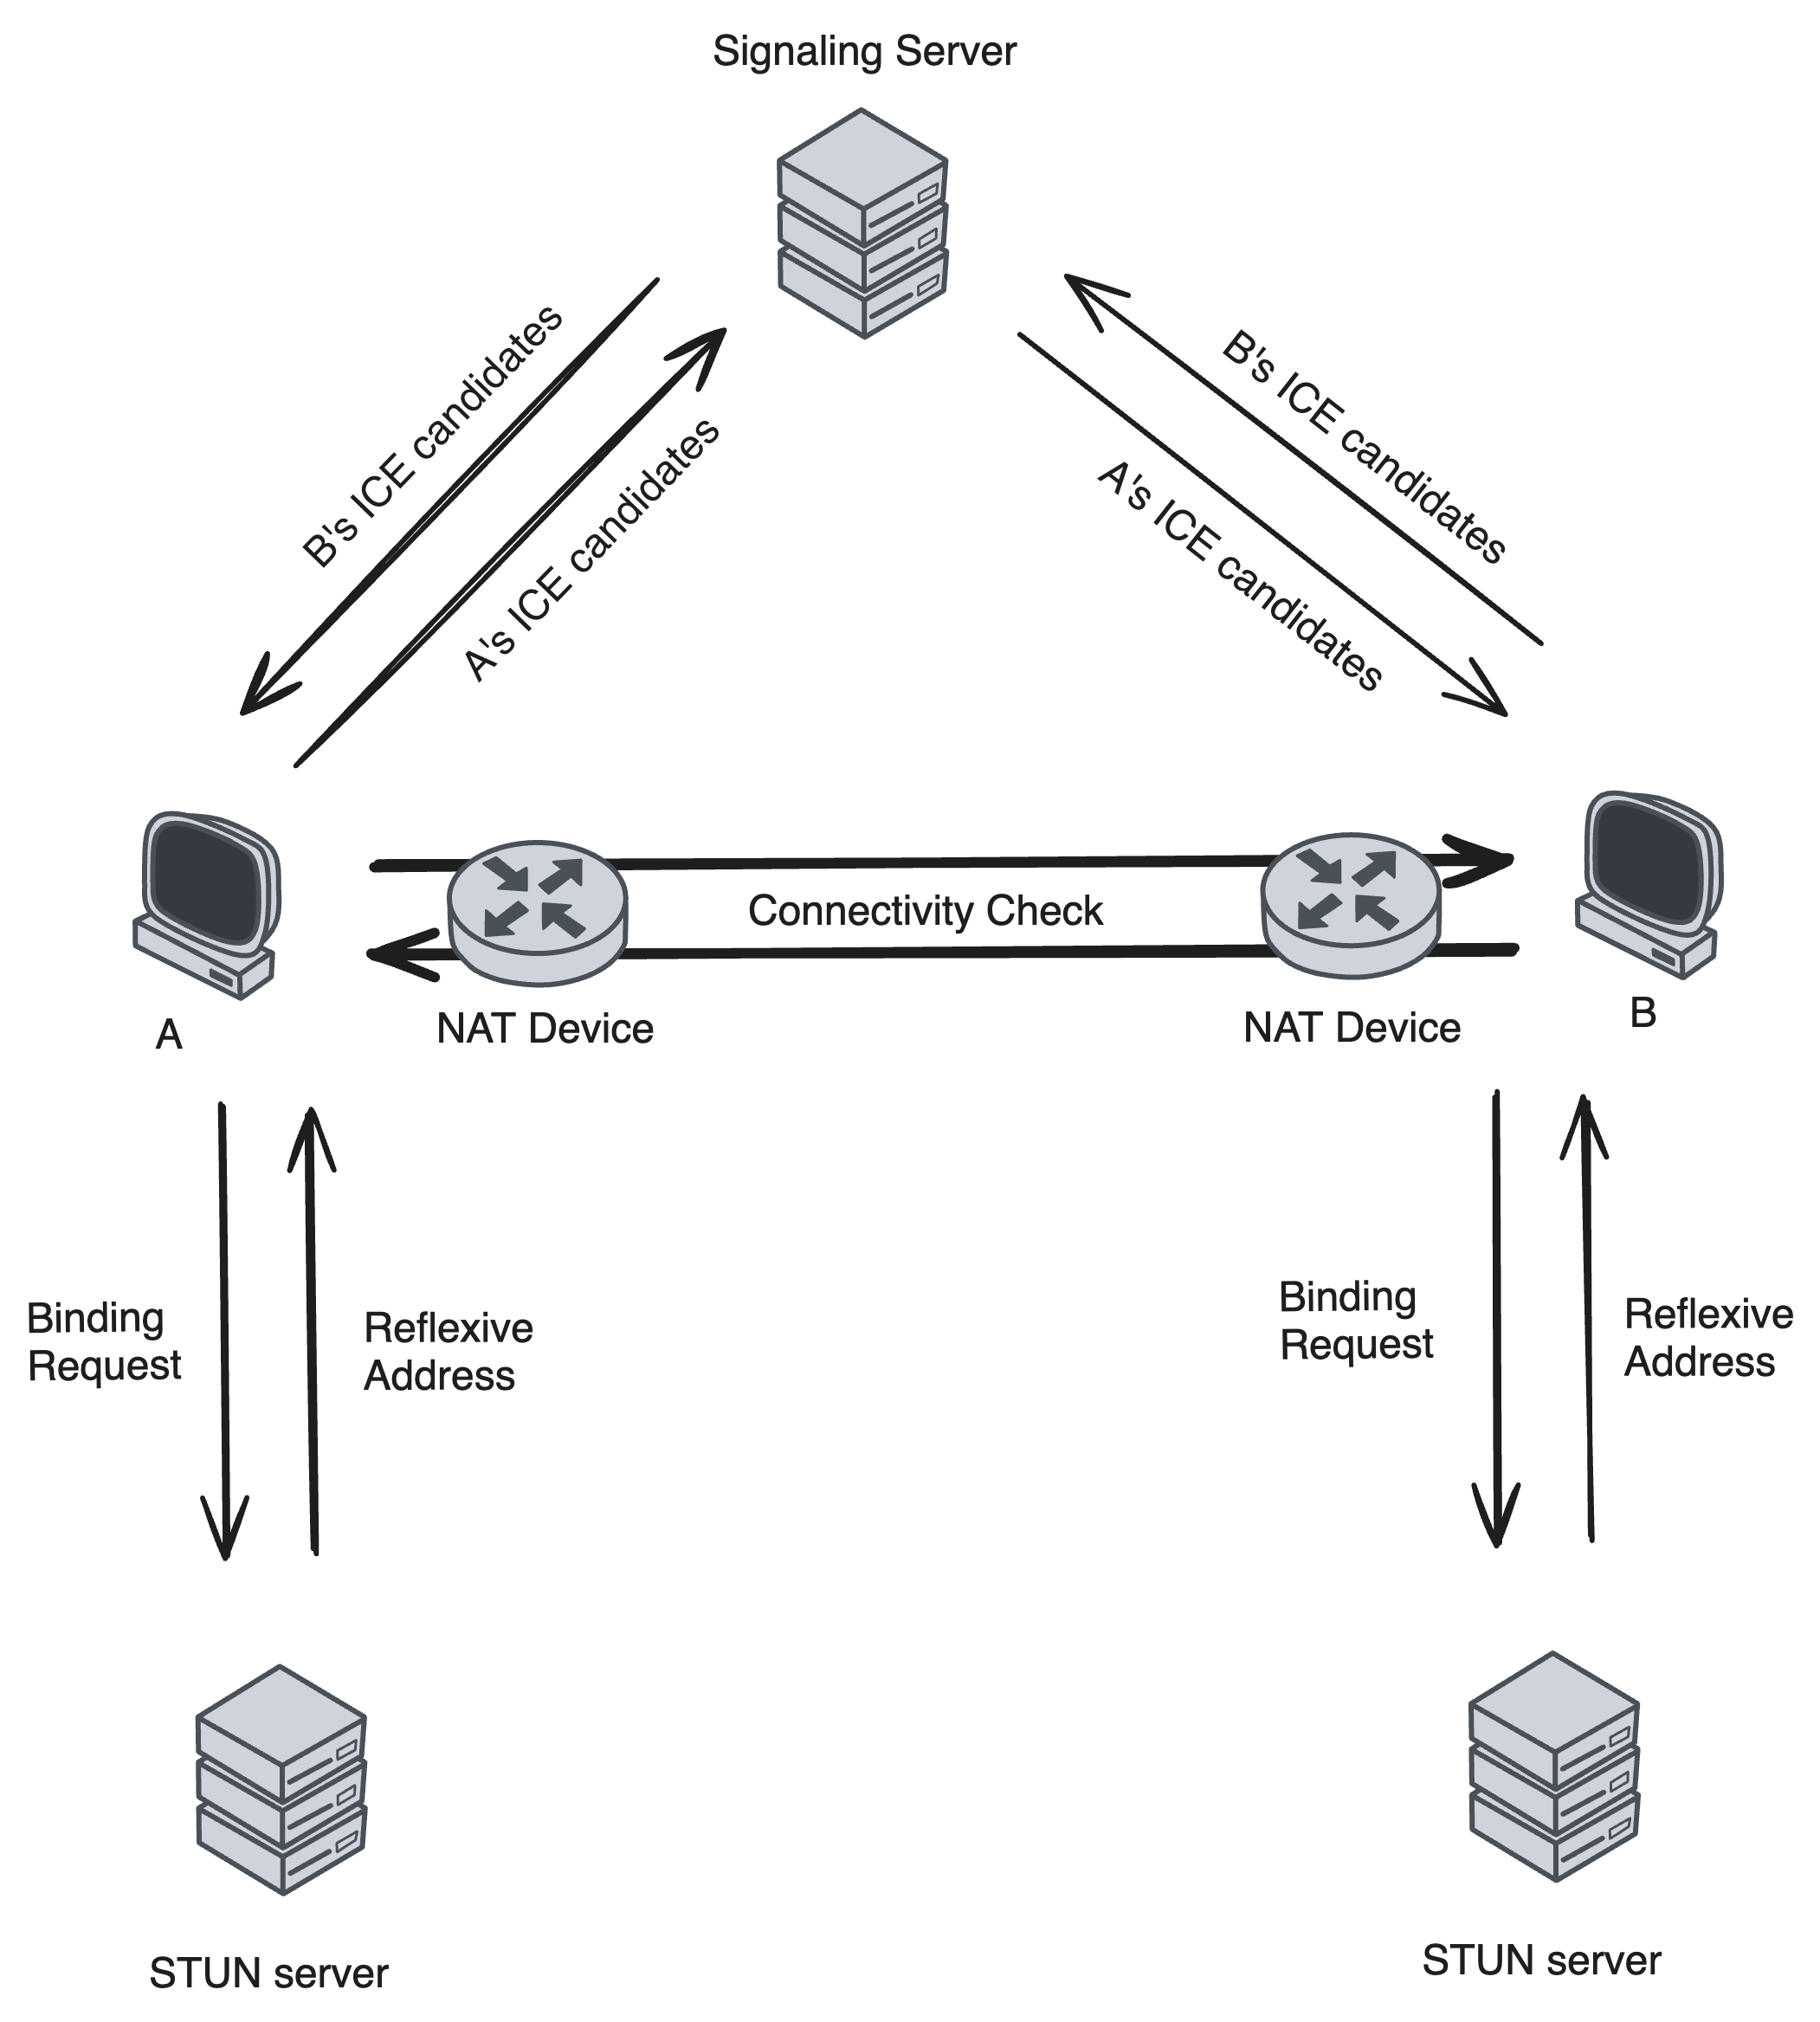
\includegraphics[width=\linewidth]{figs/ice.png}
  \caption{ICEプロトコルによるP2P通信確立の手順}
  \label{fig:ice}
\end{figure}
UDPにおいて,最適なアドレスペアの選択,NAT越えの手順,失敗時のフォールバックなどP2P通信の確立に必要な仕組みを定義した包括的なプロトコルとしてInteractive Connectivity Establishment(ICE)\cite{rfc8445}が定義されている.ICEプロトコルはWebブラウザでのリアルタイム通信プロトコルWebRTC\cite{webrtc}でも利用されており,多くのP2P通信を利用するアプリケーションはICEプロトコルに基づいている.ICEプロトコルによるP2P通信確立の手順を図~\ref{fig:ice}に示す.

\subsection{その他の先行事例}
ICEプロトコルをTCPに応用したTCP Candidates with ICE\cite{rfc6544}が定義されている.

2023年7月にはQUIC上でP2P通信を確立するための包括的なプロトコルP2P QUIC\cite{p2p_quic}のドラフトがIETFに提出されたが,2024年1月に期限切れになっている.

\section{提案されている手法}
本稿で実装する,Using QUIC to traverse NATsで提案されているP2P通信の確立手法は以下の二つである.

\subsection{手法1: ICEプロトコルを用いた通信確立}
先行事例で示したICEプロトコルを用いてUDP上でP2P通信を確立し,その通信の上でQUICハンドシェイクを開始する.QUICはUDPの上に成り立つプロトコルであるためこの手法は成立する.

この手法は既存のICEプロトコル実装を利用でき,またQUIC自体の変更は必要ないためプロトコルを拡張できない環境でのユースケースが想定される.

\subsection{手法2: QUICのみを用いた通信確立}
この手法ではICEプロトコルが司るアドレス交換や接続性チェックを全てQUICプロトコルの上で行う.アドレスペアの優先順位を決定するアルゴリズムや通信確立の手順はICEプロトコルを踏襲するため,ICE over QUICの実装とも言える.接続性チェックに関しては,QUICのハンドシェイクに含まれるPath Validationフレームを用いる.これにより,接続性チェックとハンドシェイクを併せて行うことができ,手法1に比べて通信確立がより効率的になる.

一方で,既存のICEプロトコルの実装は使えないため,実装の際はICEプロトコルをQUIC上で再実装する必要がある.またQUICの拡張が必要なため,プロトコルの拡張ができない環境ではこの手法を利用することはできない.

\section{実装}
前章で示した二つの手法について,プログラミング言語Pythonを用いて実装を行なった.また両手法についてQUICライブラリaioquic\cite{aioquic}を使用し,手法1についてはICEライブラリaioice\cite{aioice}を使用した.

本稿での実装は\url{https://github.com/kota-yata/2023f-wip}に公開している.

\subsection{手法1の実装}

ICEプロトコルを用いて確立したP2P通信をQUICに再利用する際,通信に使われるソケットを再利用する必要がある.aioice,aioquicともにソケットにライブラリ外部からアクセスする機能は存在しなかったため,aioiceについてはソケットを取り出す処理,aioquicについては接続開始時にソケットを引数として渡す処理を追加し拡張した.

aioiceで通信を確立する際にアドレスペアを交換するための仲介サーバーが必要になるが,これもPythonを用いてWebSocketで通信を行うサーバーを実装した.

\subsection{手法2の実装}
\begin{figure}[h]
  \centering
  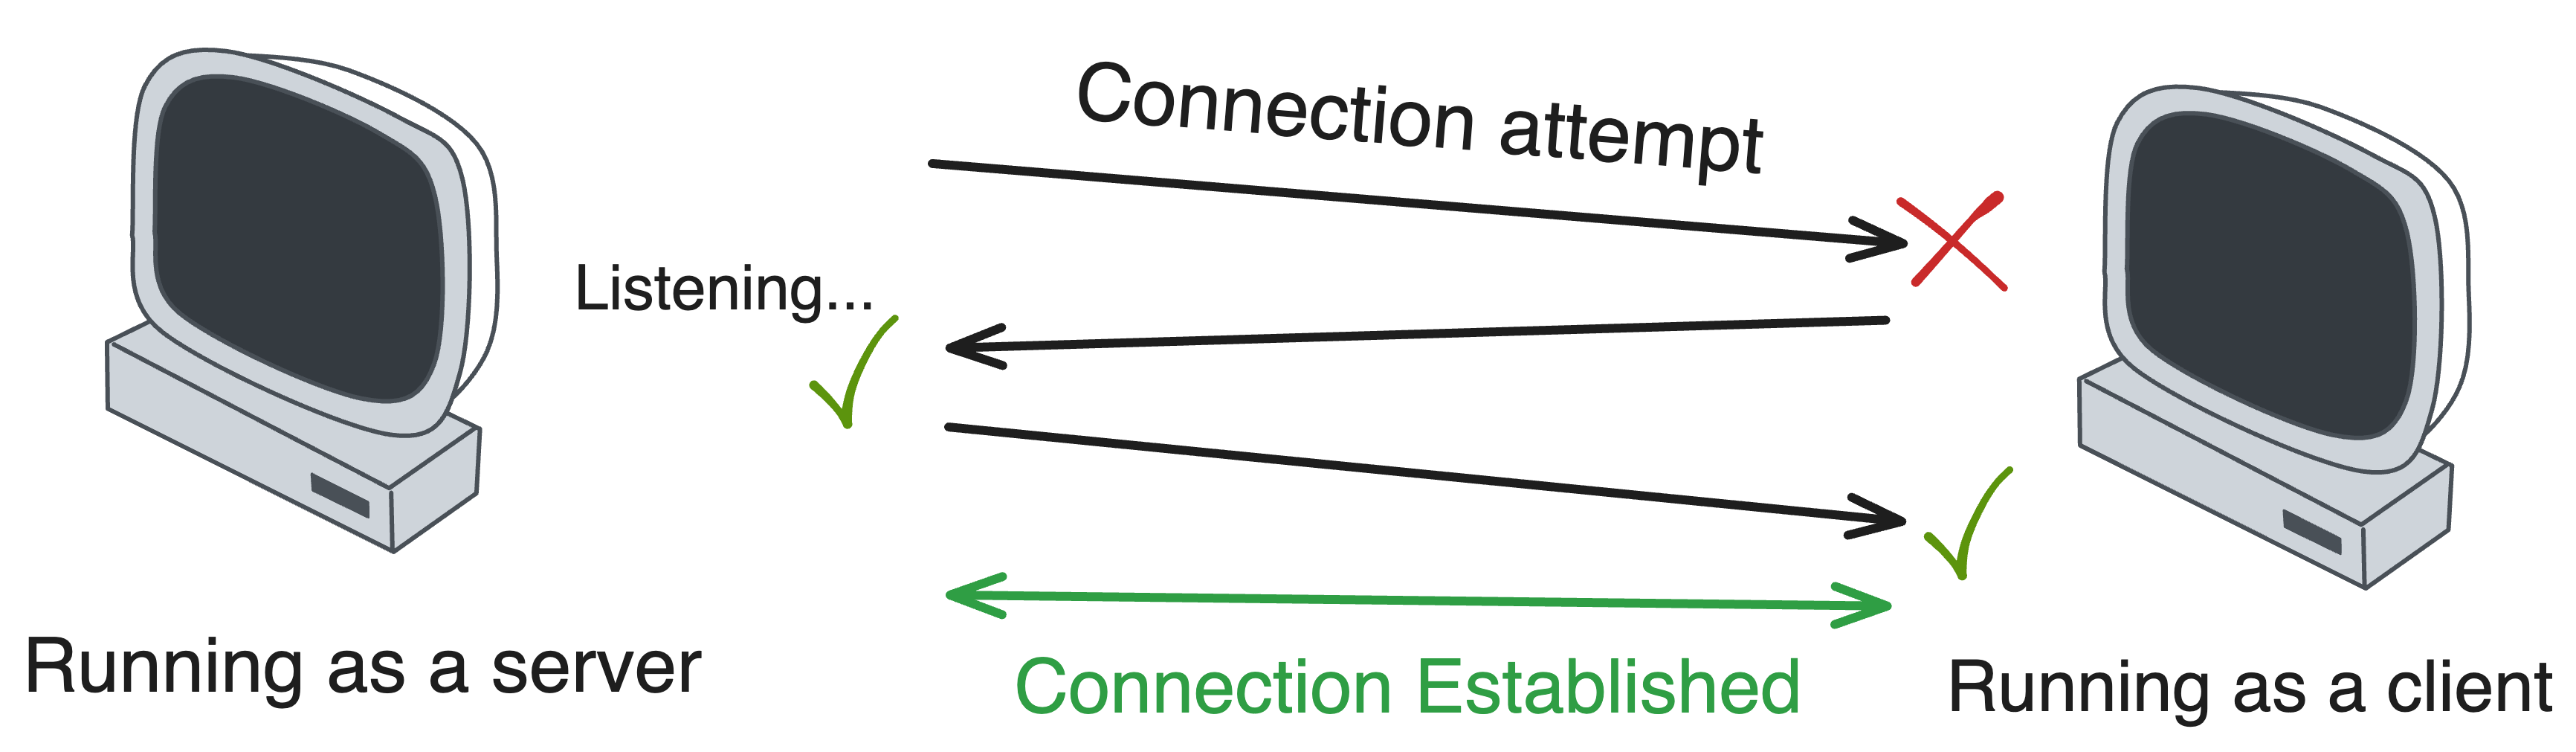
\includegraphics[width=\linewidth]{figs/implement-2.png}
  \caption{QUIC上でのNAT越え}
  \label{fig:impl-2}
\end{figure}
手法2においても,手法1同様にaioquicについて接続開始時にソケットを引数として渡す処理を追加した.また,QUICでは接続開始できるのはクライアント側のみと定義されているが,手法2ではサーバー側からPath Validationフレームを送信する必要があるため,サーバー側からも接続開始できるように拡張をした.

Using QUIC to traverse NATsで提案されているようなICE over QUICの再実装を全て完了することができなかったため,本稿の実装では双方のIPアドレスとポート番号を決め打ちで指定し,Path Validationを送り合ってNAT越えを実現する部分を実装範囲とした.具体的には図~\ref{fig:impl-2}に示すように,片方のピアは接続試行しつつサーバーとして接続を受け付け,もう片方のピアは接続試行を行う.双方から接続試行を行うことで双方のNATデバイスでマッピングが行われ,NAT越えが成立する.本来ICE over QUICが実装できている状態であれば,ICEプロトコルの最初の手順であるSTUNサーバーへの問い合わせの時点でNATマッピングが行われるが,今回はアドレス交換などを省くため図~\ref{fig:impl-2}に示したようなホールパンチングを行った.

\section{実験}
手法1について,通信確立の確認と,UDPでのP2P通信確立時との速度の比較を行った.手法2については他手法と比較を行う程度まで実装が及ばなかったため,前章で示したNAT越えで通信が確立したことを確認した

\subsection{実行環境}
両手法の実行について,片方のピアはMac OS 13.5 (Ventura),片方はGoogle CloudのCompute Engineを利用し,Ubuntu 18.0.4の仮想マシンを利用した.双方ともローカルネットワーク内に存在し,NATタイプはFull-Cone NATである.手法1で利用する仲介サーバーはHerokuにデプロイして実行した.

通信を確認するためのパケットキャプチャはWireshark 4.2.2を利用した.

\subsection{手法1の実験}
\subsubsection{通信確立の確認}
\begin{figure}[h]
  \centering
  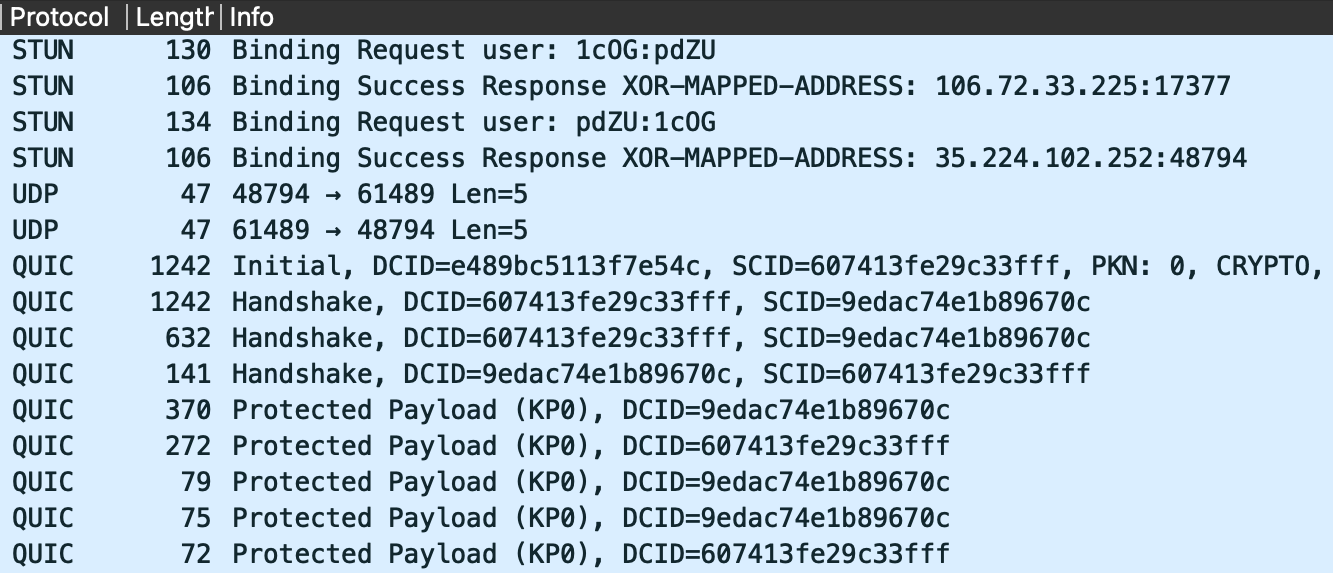
\includegraphics[width=\linewidth]{figs/ice-eva.png}
  \caption{手法1の実行結果}
  \label{fig:eva-1}
\end{figure}

手法1の通信確立が確認できた際のピア間のパケットキャプチャの様子を図~\ref{fig:eva-1}に示す.STUNパケットを用いた接続性チェックの後,QUICでのハンドシェイクが始まり,その後通信が確立されている.
\subsubsection{UDPでのP2P通信確立のみとの比較}
UDPでのP2P通信確立は単にICEプロトコルを用いて行った.手法1はICEプロトコルでの通信確立の後にQUICハンドシェイクを行っているため,UDPでの通信確立に比べて速度が遅くなることは自明である.

比較は,手法1を30回実行し,ICEプロトコルの通信が確立するまでの秒数,その後のQUICハンドシェイクまで含めた秒数をそれぞれ計測し平均を算出した.

ICEプロトコルの通信が確立するまでは平均で約4.82秒,その後のQUICハンドシェイクまで含めると約5.35秒であった.つまりQUICのハンドシェイクには約0.5秒かかっていることになる.

\subsection{手法2の実験}
\begin{figure}[h]
  \centering
  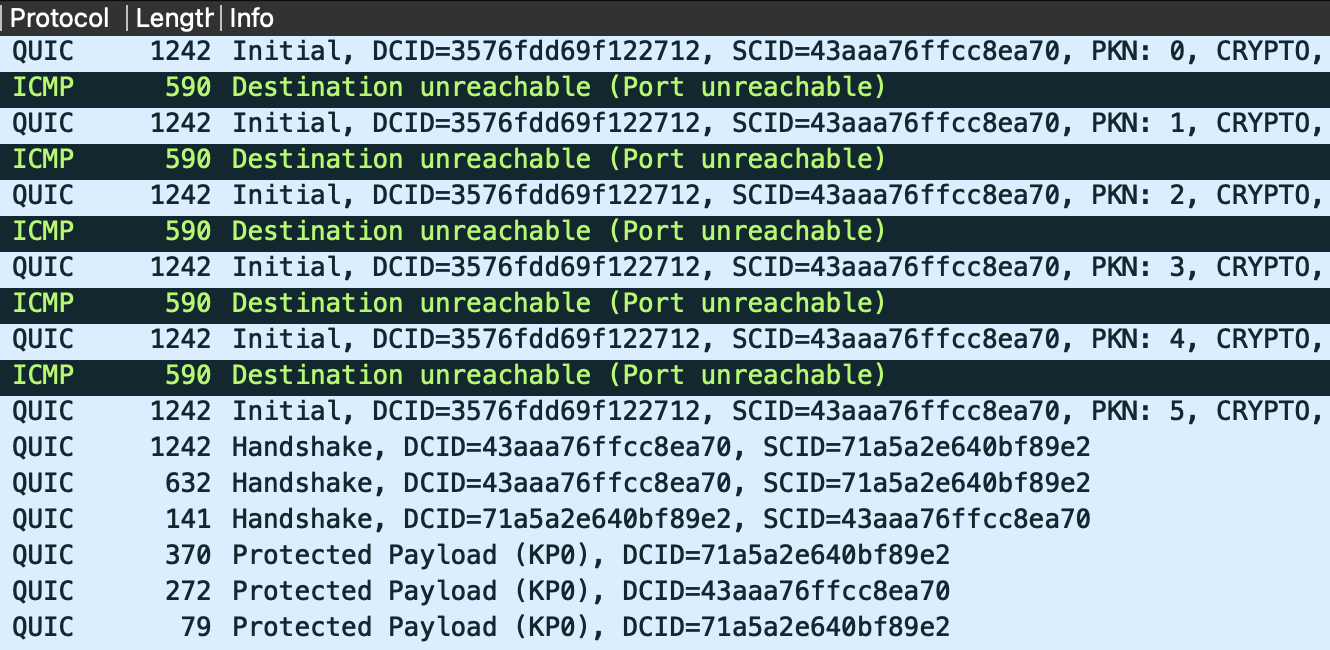
\includegraphics[width=\linewidth]{figs/quic-eva.png}
  \caption{手法2の実行結果}
  \label{fig:eva-2}
\end{figure}

手法2の通信確立が確認できた際のピア間のパケットキャプチャの様子を図~\ref{fig:eva-2}に示す.クライアント側が接続を開始しても,サーバー側のNATマッピングがなされていない最初の数回の試行はDestination unreachableで失敗している.その後NAT越えが成功し,通信が確立している.

手法2が完全に実装できた際の評価などは次章で述べる.

\section{今後の計画}
本稿では,手法2の実装を完了することができなかった.手法2を実装し,ICE over QUICが実現すれば,手法1は元より先行事例で示した他プロトコルでのNAT越えやUDP上での純粋なICEプロトコルとの定量的な比較が可能になる.手法1との比較については特に,3章で述べたように論理的には手法2の方が通信確立は効率的だが,実際に実験を行なって速度を確認することができる.

手法2の実装と併せて,QUIC上の他プロトコルの実装も今後の計画の一つである.今回aioiceとaioquicを拡張したが,その際に両ライブラリとPythonの非同期処理に関する知識を多く得ることができた.これを生かしてQUICやP2P通信に関するプロトコルの実装,議論に参加していく.

\section{結論}
QUIC上でP2P通信を確立する手法はこれまで仕様として提案されておらず,Using QUIC to traverse NATsで初めて提案された.しかし提案された手法は実装が公開されていなかったため,QUICプロトコルへの理解,実装力の向上を目的として実装を行なった.最終的に提案手法に完全に沿った実装は間に合わなかったが、QUIC上でのP2P通信は確認することができた.提案されている2つの手法の比較や定量的な評価は今後の計画とする.


% ref.bibに追記していってもいいが,mendeleyアカウントを持っているなら,overleafのupload bib from mendeleyの機能を使った方が効率的.
\bibliographystyle{unsrt}
\bibliography{ref}

\end{document}